\begin{appendices}
	
\chapter{Node28}
\label{app:node28}
\begin{figure}[h]
    \centering
    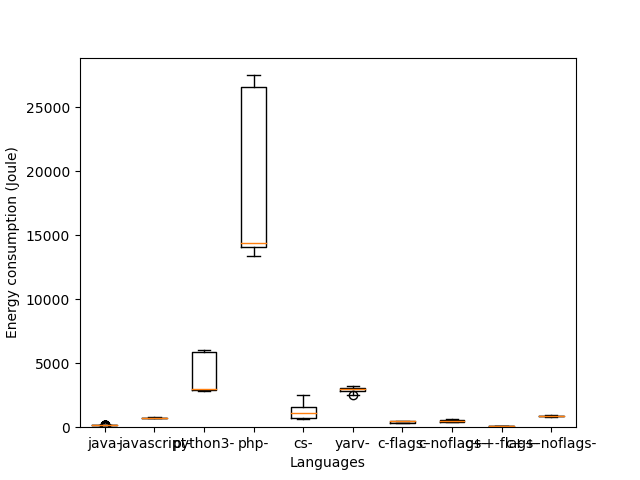
\includegraphics[width=.6\textwidth]{graphs/binarytrees_BOXoverview3.png}
    \caption{The box plot of the different programs in a programming language for the problem Binarytrees on \textit{node28}.}
    \label{fig:box-binarytrees3}
\end{figure}

\begin{table}[h]
\centering
\resizebox{\textwidth}{!}{%
\begin{tabular}{|l|c|c|c|c|c|c|c|c|c|c|}
\hline
 & \multicolumn{1}{l|}{Java} & \multicolumn{1}{l|}{JavaScript} & \multicolumn{1}{l|}{Python} & \multicolumn{1}{l|}{PHP} & \multicolumn{1}{l|}{C\#} & \multicolumn{1}{l|}{Ruby} & \multicolumn{1}{l|}{C-flags} & \multicolumn{1}{l|}{C-noflags} & \multicolumn{1}{l|}{C++-flags} & \multicolumn{1}{l|}{C++-noflags} \\ \hline
Java & 0 & + & + & + & + & + & + & + & - & +\\ \hline
JavaScript & - & 0 & + & + & + & + & - & - & - & +\\ \hline
Python & - & - & 0 & + & - & - & - & - & - & -\\ \hline
PHP & - & - & - & 0 & - & - & - & - & - & -\\ \hline
C\# & - & - & + & + & 0 & + & - & - & - & -\\ \hline
Ruby & - & - & + & + & - & 0 & - & - & - & -\\ \hline
C-flags & - & + & + & + & + & + & 0 & + & - & +\\ \hline
C-noflags & - & + & + & + & + & + & - & 0 & - & +\\ \hline
C++-flags & + & + & + & + & + & + & + & + & 0 & +\\ \hline
C++-noflags & - & - & + & + & + & + & - & - & - & 0\\ \hline
\end{tabular}%
}
\caption{The comparison of the different languages for the Binarytrees problem on \textit{node28}. A \textit{+} means that the language on the row has a lower energy consumption then the language on the column, the opposite for \textit{-}.}
\label{tab:lang-binarytrees3}
\end{table}

\begin{figure}[h]
    \centering
    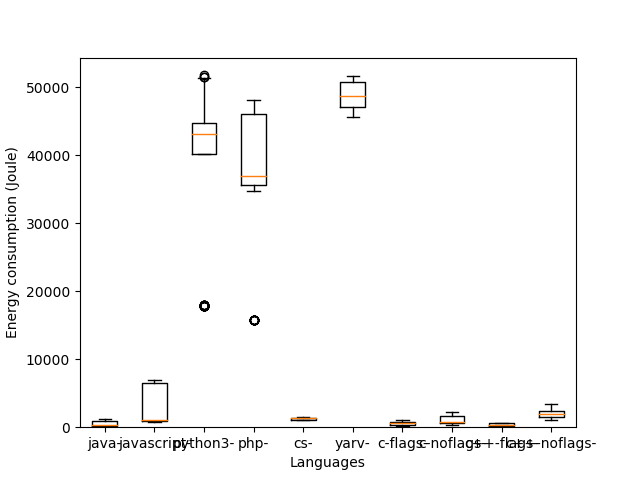
\includegraphics[width=.6\textwidth]{graphs/fannkuchredux_BOXoverview3.png}
    \caption{The box plot of the different programs in a programming language for the problem Fannkuchredux on \textit{node28}.}
    \label{fig:box-fannkuchredux3}
\end{figure}

\begin{table}[h]
\centering
\resizebox{\textwidth}{!}{%
\begin{tabular}{|l|c|c|c|c|c|c|c|c|c|c|}
\hline
 & \multicolumn{1}{l|}{Java} & \multicolumn{1}{l|}{JavaScript} & \multicolumn{1}{l|}{Python} & \multicolumn{1}{l|}{PHP} & \multicolumn{1}{l|}{C\#} & \multicolumn{1}{l|}{Ruby} & \multicolumn{1}{l|}{C-flags} & \multicolumn{1}{l|}{C-noflags} & \multicolumn{1}{l|}{C++-flags} & \multicolumn{1}{l|}{C++-noflags} \\ \hline
Java & 0 & + & + & + & + & + & + & + & + & + \\ \hline
JavaScript & - & 0 & + & + & + & + & - & - & - & + \\ \hline
Python & - & - & 0 & - & - & + & - & - & - & - \\ \hline
PHP & - & - & + & 0 & - & + & - & - & - & - \\ \hline
C\# & - & - & + & + & 0 & + & - & - & - & +\\ \hline
Ruby & - & - & - & - & - & 0 & - & - & - & -\\ \hline
C-flags & - & + & + & + & + & + & 0 & + & - & +\\ \hline
C-noflags & - & + & + & + & + & + & - & 0 & - & +\\ \hline
C++-flags & - & + & + & + & + & + & + & + & 0 & +\\ \hline
C++-noflags & - & - & + & + & - & + & - & - & - & 0\\ \hline
\end{tabular}%
}
\caption{The comparison of the different languages for the Fannkuchredux problem on \textit{node28}. A \textit{+} means that the language on the row has a lower energy consumption then the language on the column, the opposite for \textit{-}.}
\label{tab:lang-fannkuchredux3}
\end{table}

\begin{figure}[h]
    \centering
    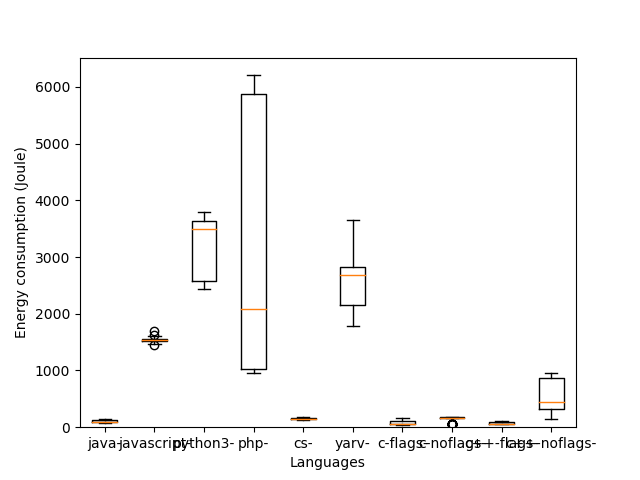
\includegraphics[width=.6\textwidth]{graphs/fasta_BOXoverview3.png}
    \caption{The box plot of the different programs in a programming language for the problem Fasta on \textit{node28}.}
    \label{fig:box-fasta3}
\end{figure}

% Please add the following required packages to your document preamble:
% \usepackage{graphicx}
\begin{table}[h]
\centering
\resizebox{\textwidth}{!}{%
\begin{tabular}{|l|c|c|c|c|c|c|c|c|c|c|}
\hline
 & \multicolumn{1}{l|}{Java} & \multicolumn{1}{l|}{JavaScript} & \multicolumn{1}{l|}{Python} & \multicolumn{1}{l|}{PHP} & \multicolumn{1}{l|}{C\#} & \multicolumn{1}{l|}{Ruby} & \multicolumn{1}{l|}{C-flags} & \multicolumn{1}{l|}{C-noflags} & \multicolumn{1}{l|}{C++-flags} & \multicolumn{1}{l|}{C++-noflags} \\ \hline
Java & 0 & + & + & + & + & + & - & + & - & + \\ \hline
JavaScript & - & 0 & + & + & - & + & - & - & - & - \\ \hline
Python & - & - & 0 & - & - & - & - & - & - & - \\ \hline
PHP & - & - & + & 0 & - & + & - & - & - & - \\ \hline
C\# & - & + & + & + & 0 & + & - & + & - & + \\ \hline
Ruby & - & - & + & - & - & 0 & - & - & - & - \\ \hline
C-flags & + & + & + & + & + & + & 0 & + & + & + \\ \hline
C-noflags & - & + & + & + & - & + & - & 0 & - & + \\ \hline
C++-flags & + & + & + & + & + & + & - & + & 0 & + \\ \hline
C++-noflags & - & + & + & + & - & + & - & - & - & 0 \\ \hline
\end{tabular}%
}
\caption{The comparison of the different languages for the Fasta problem on \textit{node28}. A \textit{+} means that the language on the row has a lower energy consumption then the language on the column, the opposite for \textit{-}.}
\label{tab:lang-fasta3}
\end{table}

\begin{figure}[h]
    \centering
    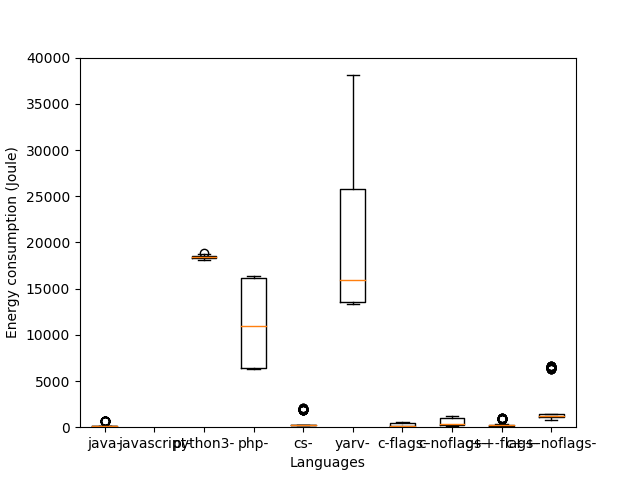
\includegraphics[width=.6\textwidth]{graphs/mandelbrot_BOXoverview3.png}
    \caption{The box plot of the different programs in a programming language for the problem Mandelbrot on \textit{node28}.}
    \label{fig:box-mandelbrot3}
\end{figure}

% Please add the following required packages to your document preamble:
% \usepackage{graphicx}
\begin{table}[h]
\centering
\resizebox{\textwidth}{!}{%
\begin{tabular}{|l|c|c|c|c|c|c|c|c|c|c|}
\hline
 & \multicolumn{1}{l|}{Java} & \multicolumn{1}{l|}{JavaScript} & \multicolumn{1}{l|}{Python} & \multicolumn{1}{l|}{PHP} & \multicolumn{1}{l|}{C\#} & \multicolumn{1}{l|}{Ruby} & \multicolumn{1}{l|}{C-flags} & \multicolumn{1}{l|}{C-noflags} & \multicolumn{1}{l|}{C++-flags} & \multicolumn{1}{l|}{C++-noflags} \\ \hline
Java & 0 & & + & + & + & + & - & + & - & +\\ \hline
JavaScript & & & & & & & & & & \\ \hline
Python& - & & 0 & - & - & Unknown & - & - & - & -\\ \hline
PHP & - & & + & 0 & - & + & - & - & - & -\\ \hline
C\# & - & & + & + & 0 & + & - & Unknown & - & +\\ \hline
Ruby & - & & Unknown & - & - & 0 & - & - & - & -\\ \hline
C-flags & + & & + & + & + & + & 0 & + & Unknown & +\\ \hline
C-noflags & - & & + & + & Unknown & + & - & 0 & - & +\\ \hline
C++-flags & + & & + & + & + & + & Unknown & + & 0 & +\\ \hline
C++-noflags & - & & + & + & - & + & - & - & - & 0\\ \hline
\end{tabular}%
}
\caption{The comparison of the different languages for the Mandelbrot problem on \textit{node28}. A \textit{+} means that the language on the row has a lower energy consumption then the language on the column, the opposite for \textit{-}, and the \textit{Unknown} means that we could not reject the null hypothesis.}
\label{tab:lang-mandelbrot3}
\end{table}

\begin{figure}[h]
    \centering
    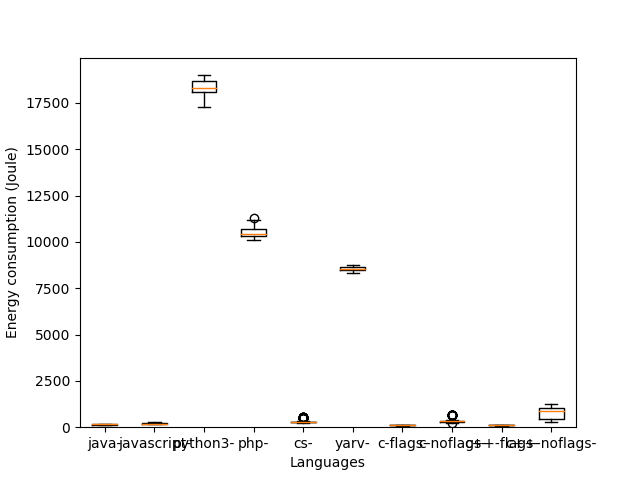
\includegraphics[width=.6\textwidth]{graphs/nbody_BOXoverview3.png}
    \caption{The box plot of the different programs in a programming language for the problem Nbody on \textit{node28}.}
    \label{fig:box-nbody3}
\end{figure}

% Please add the following required packages to your document preamble:
% \usepackage{graphicx}
\begin{table}[h]
\centering
\resizebox{\textwidth}{!}{%
\begin{tabular}{|l|c|c|c|c|c|c|c|c|c|c|}
\hline
 & \multicolumn{1}{l|}{Java} & \multicolumn{1}{l|}{JavaScript} & \multicolumn{1}{l|}{Python} & \multicolumn{1}{l|}{PHP} & \multicolumn{1}{l|}{C\#} & \multicolumn{1}{l|}{Ruby} & \multicolumn{1}{l|}{C-flags} & \multicolumn{1}{l|}{C-noflags} & \multicolumn{1}{l|}{C++-flags} & \multicolumn{1}{l|}{C++-noflags} \\ \hline
Java& 0 & + & + & + & + & + & - & + & - & +\\ \hline
JavaScript & - & 0 & + & + & + & + & - & + & - & +\\ \hline
Python& - & - & 0 & - & - & - & - & - & - & -\\ \hline
PHP & - & - & + & 0 & - & - & - & - & - & -\\ \hline
C\# & - & - & + & + & 0 & + & - & + & - & +\\ \hline
Ruby & - & - & + & + & - & 0 & - & - & - & -\\ \hline
C-flags & + & + & + & + & + & + & 0 & + & Unknown & +\\ \hline
C-noflags & - & - & + & + & - & + & - & 0 & - & +\\ \hline
C++-flags & + & + & + & + & + & + & Unknown & + & 0 & +\\ \hline
C++-noflags & - & - & + & + & - & + & - & - & - & 0\\ \hline
\end{tabular}%
}
\caption{The comparison of the different languages for the Nbody problem on \textit{node28}. A \textit{+} means that the language on the row has a lower energy consumption then the language on the column, the opposite for \textit{-}, and the \textit{Unknown} means that we could not reject the null hypothesis.}
\label{tab:lang-nbody3}
\end{table}

\begin{figure}[h]
    \centering
    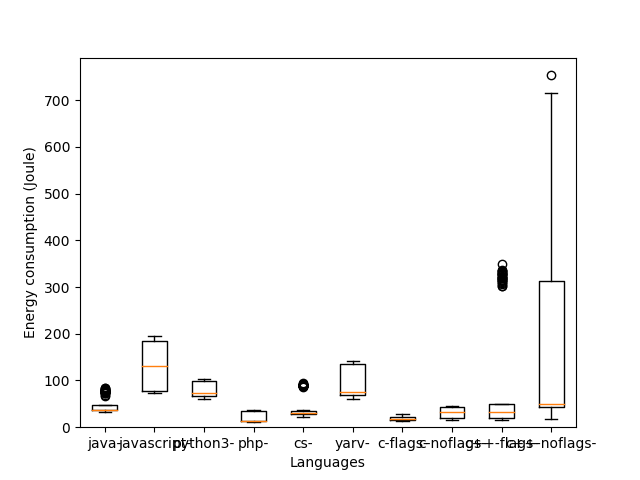
\includegraphics[width=.6\textwidth]{graphs/revcomp_BOXoverview3.png}
    \caption{The box plot of the different programs in a programming language for the problem Revcomp on \textit{node28}.}
    \label{fig:box-revcomp3}
\end{figure}

% Please add the following required packages to your document preamble:
% \usepackage{graphicx}
\begin{table}[h]
\centering
\resizebox{\textwidth}{!}{%
\begin{tabular}{|l|c|c|c|c|c|c|c|c|c|c|}
\hline
 & \multicolumn{1}{l|}{Java} & \multicolumn{1}{l|}{JavaScript} & \multicolumn{1}{l|}{Python} & \multicolumn{1}{l|}{PHP} & \multicolumn{1}{l|}{C\#} & \multicolumn{1}{l|}{Ruby} & \multicolumn{1}{l|}{C-flags} & \multicolumn{1}{l|}{C-noflags} & \multicolumn{1}{l|}{C++-flags} & \multicolumn{1}{l|}{C++-noflags} \\ \hline
Java& 0 & + & + & - & - & + & - & - & - & +\\ \hline
JavaScript& - & 0 & - & - & - & - & - & - & - & -\\ \hline
Python& - & + & 0 & - & - & + & - & - & - & -\\ \hline
PHP & + & + & + & 0 & + & + & + & + & + & +\\ \hline
C\# & + & + & + & - & 0 & + & - & Unknown & Unknown & +\\ \hline
Ruby& - & + & - & - & - & 0 & - & - & - & -\\ \hline
C-flags & + & + & + & - & + & + & 0 & + & + & +\\ \hline
C-noflags & + & + & + & - & Unknown & + & - & 0 & Unknown & +\\ \hline
C++-flags & + & + & + & - & Unknown & + & - & Unknown & 0 & +\\ \hline
C++-noflags & - & + & + & - & - & + & - & - & - & 0\\ \hline
\end{tabular}%
}
\caption{The comparison of the different languages for the Revcomp problem on \textit{node28}. A \textit{+} means that the language on the row has a lower energy consumption then the language on the column, the opposite for \textit{-}, and the \textit{Unknown} means that we could not reject the null hypothesis.}
\label{tab:lang-revcomp3}
\end{table}

\begin{figure}[h]
    \centering
    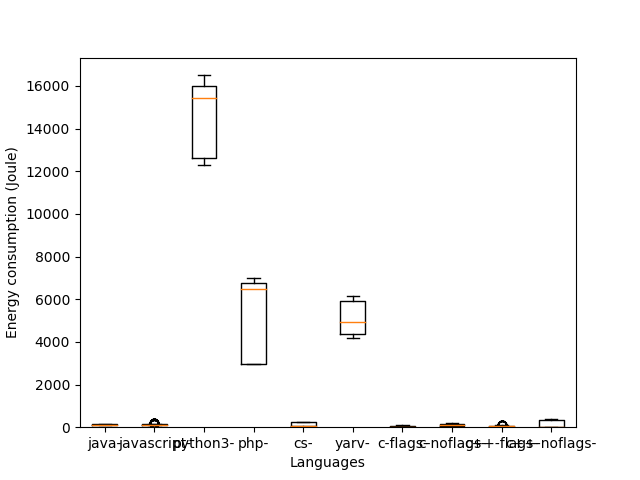
\includegraphics[width=.6\textwidth]{graphs/spectralnorm_BOXoverview3.png}
    \caption{The box plot of the different programs in a programming language for the problem Spectralnorm on \textit{node29}.}
    \label{fig:box-spectralnorm3}
\end{figure}

% Please add the following required packages to your document preamble:
% \usepackage{graphicx}
\begin{table}[h]
\centering
\resizebox{\textwidth}{!}{%
\begin{tabular}{|l|c|c|c|c|c|c|c|c|c|c|}
\hline
 & \multicolumn{1}{l|}{Java} & \multicolumn{1}{l|}{JavaScript} & \multicolumn{1}{l|}{Python} & \multicolumn{1}{l|}{PHP} & \multicolumn{1}{l|}{C\#} & \multicolumn{1}{l|}{Ruby} & \multicolumn{1}{l|}{C-flags} & \multicolumn{1}{l|}{C-noflags} & \multicolumn{1}{l|}{C++-flags} & \multicolumn{1}{l|}{C++-noflags} \\ \hline
Java& 0 & - & + & + & Unknown & + & - & - & - & -\\ \hline
JavaScript& + & 0 & + & + & Unknown & + & - & - & - & -\\ \hline
Python& - & - & 0 & - & - & - & - & - & - & -\\ \hline
PHP & - & - & + & 0 & - & Unknown & - & - & - & -\\ \hline
C\# & Unknown & Unknown & + & + & 0 & + & - & Unknown & - & Unknown\\ \hline
Ruby& - & - & + & Unknown & - & 0 & - & - & - & -\\ \hline
C-flags & + & + & + & + & + & + & 0 & + & + & +\\ \hline
C-noflags & + & + & + & + & Unknown & + & - & 0 & - & -\\ \hline
C++-flags & + & + & + & + & + & + & - & + & 0 & +\\ \hline
C++-noflags & + & + & + & + & Unknown & + & - & + & - & 0\\ \hline
\end{tabular}%
}
\caption{The comparison of the different languages for the Spectralnorm problem on \textit{node28}. A \textit{+} means that the language on the row has a lower energy consumption then the language on the column, the opposite for \textit{-}, and the \textit{Unknown} means that we could not reject the null hypothesis.}
\label{tab:lang-spectralnorm3}
\end{table}

\begin{table}[h]
\centering
\begin{tabular}{|l|l|l|l|}
\hline
Program 1 & Program 2 & p-less & p-greater \\ \hline
java-3.problem0 & java-6.problem0 & 0.266 & 0.740 \\ \hline
javascript-1.problem2 & javascript-2.problem2 & 0.829 & 0.176 \\ \hline
javascript-1.problem2 & javascript-3.problem2 & 0.413 & 0.594 \\ \hline
javascript-2.problem2 & javascript-3.problem2 & 0.197 & 0.808 \\ \hline
javascript-1.problem6 & javascript-3.problem6 & 0.532 & 0.475 \\ \hline
javascript-1.problem6 & javascript-5.problem6 & 0.272 & 0.734 \\ \hline
javascript-3.problem6 & javascript-5.problem6 & 0.243 & 0.763 \\ \hline
python3-2.problem3 & python3-5.problem3 & 0.488 & 0.520 \\ \hline
cs-3.problem3 & cs-4.problem3 & 0.088 & 0.915 \\ \hline
cs-3.problem4 & cs-5.problem4 & 0.622 & 0.385 \\ \hline
cs-4.problem4 & cs-6.problem4 & 0.493 & 0.515 \\ \hline
c-noflags-1.problem2 & c-noflags-2.problem2 & 0.882 & 0.122 \\ \hline
c-flags-2.problem4 & c-flags-3.problem4 & 0.230 & 0.776 \\ \hline
c-noflags-1.problem4 & c-noflags-6.problem4 & 0.218 & 0.787 \\ \hline
c-flags-3.problem5 & c-flags-6.problem5 & 0.175 & 0.830 \\ \hline
c-noflags-4.problem5 & c-noflags-5.problem5 & 0.090 & 0.912 \\ \hline
c++-flags-1.problem0 & c++-flags-8.problem0 & 0.571 & 0.436 \\ \hline
c++-noflags-1.problem0 & c++-noflags-3.problem0 & 0.883 & 0.121 \\ \hline
c++-noflags-1.problem0 & c++-noflags-8.problem0 & 0.874 & 0.130 \\ \hline
c++-noflags-3.problem0 & c++-noflags-8.problem0 & 0.453 & 0.555 \\ \hline
c++-flags-1.problem2 & c++-flags-2.problem2 & 0.317 & 0.690 \\ \hline
c++-flags-3.problem4 & c++-flags-8.problem4 & 0.168 & 0.837 \\ \hline
c++-flags-4.problem4 & c++-flags-6.problem4 & 0.225 & 0.781 \\ \hline
c++-noflags-5.problem6 & c++-noflags-6.problem6 & 0.374 & 0.633 \\ \hline
\end{tabular}
\caption{The programs result from \textit{node28} where the null hypothesis that they are from the same distribution could not be reject for the Mann Whitney U one-sided test less and bigger.}
\label{tab:programs_equal3}
\end{table}

%------------------------------------------------------------------
%------------------------------------------------------------------
%------------------------------------------------------------------
%------------------------------------------------------------------
%--------------------HERE TO NEXT CHAPTER--------------------------
%------------------------------------------------------------------
%------------------------------------------------------------------
%------------------------------------------------------------------
%------------------------------------------------------------------

\chapter{Node29}
\label{app:node29}
\begin{figure}[h]
    \centering
    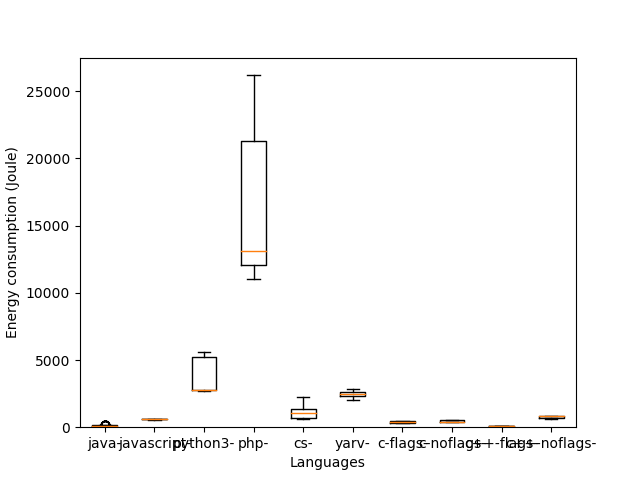
\includegraphics[width=.6\textwidth]{graphs/binarytrees_BOXoverview2.png}
    \caption{The box plot of the different programs in a programming language for the problem Binarytrees on \textit{node29}.}
    \label{fig:box-binarytrees2}
\end{figure}

\begin{table}[h]
\centering
\resizebox{\textwidth}{!}{%
\begin{tabular}{|l|c|c|c|c|c|c|c|c|c|c|}
\hline
 & \multicolumn{1}{l|}{Java} & \multicolumn{1}{l|}{JavaScript} & \multicolumn{1}{l|}{Python} & \multicolumn{1}{l|}{PHP} & \multicolumn{1}{l|}{C\#} & \multicolumn{1}{l|}{Ruby} & \multicolumn{1}{l|}{C-flags} & \multicolumn{1}{l|}{C-noflags} & \multicolumn{1}{l|}{C++-flags} & \multicolumn{1}{l|}{C++-noflags} \\ \hline
Java & 0 & + & + & + & + & + & + & + & - & +\\ \hline
JavaScript & - & 0 & + & + & + & + & - & - & - & +\\ \hline
Python & - & - & 0 & + & - & - & - & - & - & -\\ \hline
PHP & - & - & - & 0 & - & - & - & - & - & -\\ \hline
C\# & - & - & + & + & 0 & + & - & - & - & -\\ \hline
Ruby & - & - & + & + & - & 0 & - & - & - & -\\ \hline
C-flags & - & + & + & + & + & + & 0 & + & - & +\\ \hline
C-noflags & - & + & + & + & + & + & - & 0 & - & +\\ \hline
C++-flags & + & + & + & + & + & + & + & + & 0 & +\\ \hline
C++-noflags & - & - & + & + & + & + & - & - & - & 0\\ \hline
\end{tabular}%
}
\caption{The comparison of the different languages for the Binarytrees problem on \textit{node29}. A \textit{+} means that the language on the row has a lower energy consumption then the language on the column, the opposite for \textit{-}.}
\label{tab:lang-binarytrees2}
\end{table}

\begin{figure}[h]
    \centering
    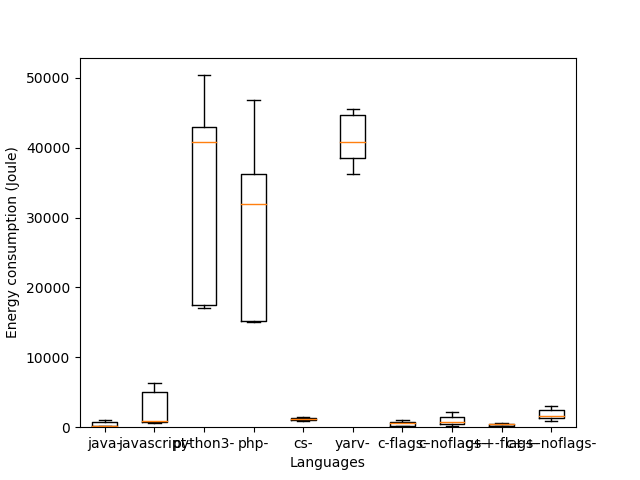
\includegraphics[width=.6\textwidth]{graphs/fannkuchredux_BOXoverview2.png}
    \caption{The box plot of the different programs in a programming language for the problem Fannkuchredux on \textit{node29}.}
    \label{fig:box-fannkuchredux2}
\end{figure}

\begin{table}[h]
\centering
\resizebox{\textwidth}{!}{%
\begin{tabular}{|l|c|c|c|c|c|c|c|c|c|c|}
\hline
 & \multicolumn{1}{l|}{Java} & \multicolumn{1}{l|}{JavaScript} & \multicolumn{1}{l|}{Python} & \multicolumn{1}{l|}{PHP} & \multicolumn{1}{l|}{C\#} & \multicolumn{1}{l|}{Ruby} & \multicolumn{1}{l|}{C-flags} & \multicolumn{1}{l|}{C-noflags} & \multicolumn{1}{l|}{C++-flags} & \multicolumn{1}{l|}{C++-noflags} \\ \hline
Java & 0 & + & + & + & + & + & + & + & Unknown & + \\ \hline
JavaScript & - & 0 & + & + & + & + & - & - & - & + \\ \hline
Python & - & - & 0 & - & - & Unknown & - & - & - & - \\ \hline
PHP & - & - & + & 0 & - & + & - & - & - & - \\ \hline
C\# & - & - & + & + & 0 & + & - & - & - & +\\ \hline
Ruby & - & - & Unknown & - & - & 0 & - & - & - & -\\ \hline
C-flags & - & + & + & + & + & + & 0 & + & - & +\\ \hline
C-noflags & - & + & + & + & + & + & - & 0 & - & +\\ \hline
C++-flags & Unknown & + & + & + & + & + & + & + & 0 & +\\ \hline
C++-noflags & - & - & + & + & - & + & - & - & - & 0\\ \hline
\end{tabular}%
}
\caption{The comparison of the different languages for the Fannkuchredux problem on \textit{node29}. A \textit{+} means that the language on the row has a lower energy consumption then the language on the column, the opposite for \textit{-}.}
\label{tab:lang-fannkuchredux2}
\end{table}

\begin{figure}[h]
    \centering
    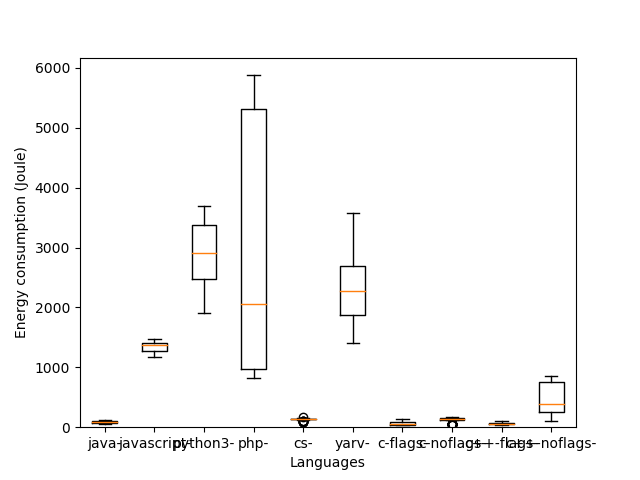
\includegraphics[width=.6\textwidth]{graphs/fasta_BOXoverview2.png}
    \caption{The box plot of the different programs in a programming language for the problem Fasta on \textit{node29}.}
    \label{fig:box-fasta2}
\end{figure}

% Please add the following required packages to your document preamble:
% \usepackage{graphicx}
\begin{table}[h]
\centering
\resizebox{\textwidth}{!}{%
\begin{tabular}{|l|c|c|c|c|c|c|c|c|c|c|}
\hline
 & \multicolumn{1}{l|}{Java} & \multicolumn{1}{l|}{JavaScript} & \multicolumn{1}{l|}{Python} & \multicolumn{1}{l|}{PHP} & \multicolumn{1}{l|}{C\#} & \multicolumn{1}{l|}{Ruby} & \multicolumn{1}{l|}{C-flags} & \multicolumn{1}{l|}{C-noflags} & \multicolumn{1}{l|}{C++-flags} & \multicolumn{1}{l|}{C++-noflags} \\ \hline
Java & 0 & + & + & + & + & + & - & + & - & + \\ \hline
JavaScript & - & 0 & + & + & - & + & - & - & - & - \\ \hline
Python & - & - & 0 & - & - & - & - & - & - & - \\ \hline
PHP & - & - & + & 0 & - & Unknown & - & - & - & - \\ \hline
C\# & - & + & + & + & 0 & + & - & Unknown & - & + \\ \hline
Ruby & - & - & + & Unknown & - & 0 & - & - & - & - \\ \hline
C-flags & + & + & + & + & + & + & 0 & + & Unknown & + \\ \hline
C-noflags & - & + & + & + & Unknown & + & - & 0 & - & + \\ \hline
C++-flags & + & + & + & + & + & + & Unknown & + & 0 & + \\ \hline
C++-noflags & - & + & + & + & - & + & - & - & - & 0 \\ \hline
\end{tabular}%
}
\caption{The comparison of the different languages for the Fasta problem on \textit{node29}. A \textit{+} means that the language on the row has a lower energy consumption then the language on the column, the opposite for \textit{-}, and the \textit{Unknown} means that we could not reject the null hypothesis.}
\label{tab:lang-fasta2}
\end{table}

\begin{figure}[h]
    \centering
    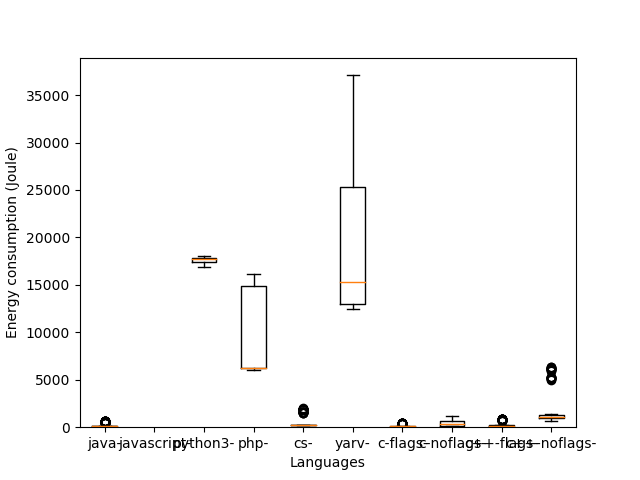
\includegraphics[width=.6\textwidth]{graphs/mandelbrot_BOXoverview2.png}
    \caption{The box plot of the different programs in a programming language for the problem Mandelbrot on \textit{node29}.}
    \label{fig:box-mandelbrot2}
\end{figure}

% Please add the following required packages to your document preamble:
% \usepackage{graphicx}
\begin{table}[h]
\centering
\resizebox{\textwidth}{!}{%
\begin{tabular}{|l|c|c|c|c|c|c|c|c|c|c|}
\hline
 & \multicolumn{1}{l|}{Java} & \multicolumn{1}{l|}{JavaScript} & \multicolumn{1}{l|}{Python} & \multicolumn{1}{l|}{PHP} & \multicolumn{1}{l|}{C\#} & \multicolumn{1}{l|}{Ruby} & \multicolumn{1}{l|}{C-flags} & \multicolumn{1}{l|}{C-noflags} & \multicolumn{1}{l|}{C++-flags} & \multicolumn{1}{l|}{C++-noflags} \\ \hline
Java & 0 & & + & + & + & + & - & + & - & +\\ \hline
JavaScript & & & & & & & & & & \\ \hline
Python& - & & 0 & - & - & - & - & - & - & -\\ \hline
PHP & - & & + & 0 & - & + & - & - & - & -\\ \hline
C\# & - & & + & + & 0 & + & - & Unknown & - & +\\ \hline
Ruby & - & & + & - & - & 0 & - & - & - & -\\ \hline
C-flags & + & & + & + & + & + & 0 & + & Unknown & +\\ \hline
C-noflags & - & & + & + & Unknown & + & - & 0 & - & +\\ \hline
C++-flags & + & & + & + & + & + & Unknown & + & 0 & +\\ \hline
C++-noflags & - & & + & + & - & + & - & - & - & 0\\ \hline
\end{tabular}%
}
\caption{The comparison of the different languages for the Mandelbrot problem on \textit{node29}. A \textit{+} means that the language on the row has a lower energy consumption then the language on the column, the opposite for \textit{-}, and the \textit{Unknown} means that we could not reject the null hypothesis.}
\label{tab:lang-mandelbrot2}
\end{table}

\begin{figure}[h]
    \centering
    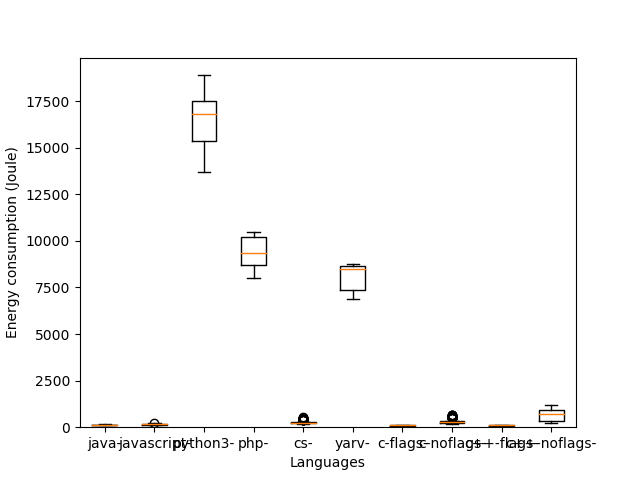
\includegraphics[width=.6\textwidth]{graphs/nbody_BOXoverview2.png}
    \caption{The box plot of the different programs in a programming language for the problem Nbody on \textit{node29}.}
    \label{fig:box-nbody2}
\end{figure}

% Please add the following required packages to your document preamble:
% \usepackage{graphicx}
\begin{table}[h]
\centering
\resizebox{\textwidth}{!}{%
\begin{tabular}{|l|c|c|c|c|c|c|c|c|c|c|}
\hline
 & \multicolumn{1}{l|}{Java} & \multicolumn{1}{l|}{JavaScript} & \multicolumn{1}{l|}{Python} & \multicolumn{1}{l|}{PHP} & \multicolumn{1}{l|}{C\#} & \multicolumn{1}{l|}{Ruby} & \multicolumn{1}{l|}{C-flags} & \multicolumn{1}{l|}{C-noflags} & \multicolumn{1}{l|}{C++-flags} & \multicolumn{1}{l|}{C++-noflags} \\ \hline
Java& 0 & + & + & + & + & + & - & + & - & +\\ \hline
JavaScript & - & 0 & + & + & + & + & - & + & - & +\\ \hline
Python& - & - & 0 & - & - & - & - & - & - & -\\ \hline
PHP & - & - & + & 0 & - & - & - & - & - & -\\ \hline
C\# & - & - & + & + & 0 & + & - & + & - & +\\ \hline
Ruby & - & - & + & + & - & 0 & - & - & - & -\\ \hline
C-flags & + & + & + & + & + & + & 0 & + & Unknown & +\\ \hline
C-noflags & - & - & + & + & - & + & - & 0 & - & +\\ \hline
C++-flags & + & + & + & + & + & + & Unknown & + & 0 & +\\ \hline
C++-noflags & - & - & + & + & - & + & - & - & - & 0\\ \hline
\end{tabular}%
}
\caption{The comparison of the different languages for the Nbody problem on \textit{node29}. A \textit{+} means that the language on the row has a lower energy consumption then the language on the column, the opposite for \textit{-}, and the \textit{Unknown} means that we could not reject the null hypothesis.}
\label{tab:lang-nbody2}
\end{table}

\begin{figure}[h]
    \centering
    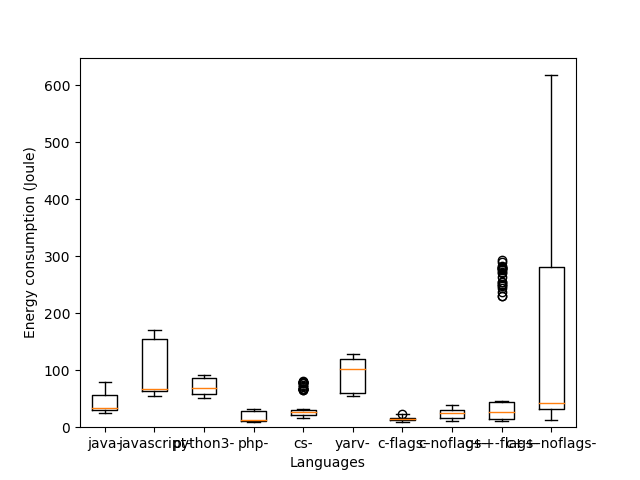
\includegraphics[width=.6\textwidth]{graphs/revcomp_BOXoverview2.png}
    \caption{The box plot of the different programs in a programming language for the problem Revcomp on \textit{node29}.}
    \label{fig:box-revcomp2}
\end{figure}

% Please add the following required packages to your document preamble:
% \usepackage{graphicx}
\begin{table}[h]
\centering
\resizebox{\textwidth}{!}{%
\begin{tabular}{|l|c|c|c|c|c|c|c|c|c|c|}
\hline
 & \multicolumn{1}{l|}{Java} & \multicolumn{1}{l|}{JavaScript} & \multicolumn{1}{l|}{Python} & \multicolumn{1}{l|}{PHP} & \multicolumn{1}{l|}{C\#} & \multicolumn{1}{l|}{Ruby} & \multicolumn{1}{l|}{C-flags} & \multicolumn{1}{l|}{C-noflags} & \multicolumn{1}{l|}{C++-flags} & \multicolumn{1}{l|}{C++-noflags} \\ \hline
Java& 0 & + & + & - & - & + & - & - & - & +\\ \hline
JavaScript& - & 0 & - & - & - & - & - & - & - & -\\ \hline
Python& - & + & 0 & - & - & + & - & - & - & -\\ \hline
PHP & + & + & + & 0 & + & + & Unknown & + & + & +\\ \hline
C\# & + & + & + & - & 0 & + & - & - & Unknown & +\\ \hline
Ruby& - & + & - & - & - & 0 & - & - & - & -\\ \hline
C-flags & + & + & + & Unknown & + & + & 0 & + & + & +\\ \hline
C-noflags & + & + & + & - & + & + & - & 0 & + & +\\ \hline
C++-flags & + & + & + & - & Unknown & + & - & - & 0 & +\\ \hline
C++-noflags & - & + & + & - & - & + & - & - & - & 0\\ \hline
\end{tabular}%
}
\caption{The comparison of the different languages for the Revcomp problem on \textit{node29}. A \textit{+} means that the language on the row has a lower energy consumption then the language on the column, the opposite for \textit{-}, and the \textit{Unknown} means that we could not reject the null hypothesis.}
\label{tab:lang-revcomp2}
\end{table}

\begin{figure}[h]
    \centering
    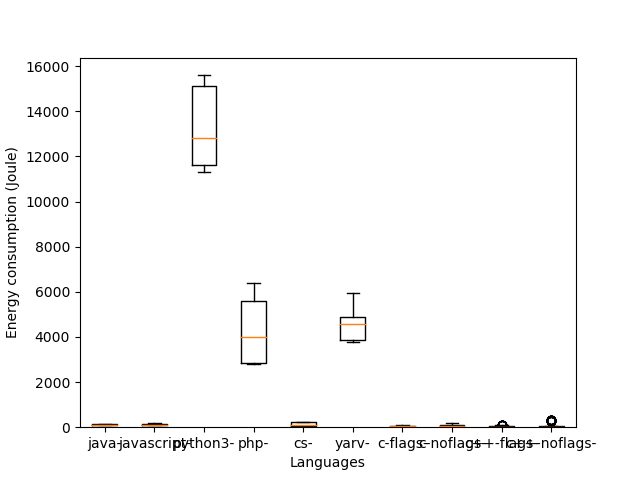
\includegraphics[width=.6\textwidth]{graphs/spectralnorm_BOXoverview2.png}
    \caption{The box plot of the different programs in a programming language for the problem Spectralnorm on \textit{node29}.}
    \label{fig:box-spectralnorm2}
\end{figure}

% Please add the following required packages to your document preamble:
% \usepackage{graphicx}
\begin{table}[h]
\centering
\resizebox{\textwidth}{!}{%
\begin{tabular}{|l|c|c|c|c|c|c|c|c|c|c|}
\hline
 & \multicolumn{1}{l|}{Java} & \multicolumn{1}{l|}{JavaScript} & \multicolumn{1}{l|}{Python} & \multicolumn{1}{l|}{PHP} & \multicolumn{1}{l|}{C\#} & \multicolumn{1}{l|}{Ruby} & \multicolumn{1}{l|}{C-flags} & \multicolumn{1}{l|}{C-noflags} & \multicolumn{1}{l|}{C++-flags} & \multicolumn{1}{l|}{C++-noflags} \\ \hline
Java& 0 & - & + & + & Unknown & + & - & - & - & -\\ \hline
JavaScript& + & 0 & + & + & Unknown & + & - & - & - & -\\ \hline
Python& - & - & 0 & - & - & - & - & - & - & -\\ \hline
PHP & - & - & + & 0 & - & Unknown & - & - & - & -\\ \hline
C\# & Unknown & Unknown & + & + & 0 & + & - & Unknown & - & Unknown\\ \hline
Ruby& - & - & + & Unknown & - & 0 & - & - & - & -\\ \hline
C-flags & + & + & + & + & + & + & 0 & + & + & +\\ \hline
C-noflags & + & + & + & + & Unknown & + & - & 0 & - & -\\ \hline
C++-flags & + & + & + & + & + & + & - & + & 0 & +\\ \hline
C++-noflags & + & + & + & + & Unknown & + & - & + & - & 0\\ \hline
\end{tabular}%
}
\caption{The comparison of the different languages for the Spectralnorm problem on \textit{node29}. A \textit{+} means that the language on the row has a lower energy consumption then the language on the column, the opposite for \textit{-}, and the \textit{Unknown} means that we could not reject the null hypothesis.}
\label{tab:lang-spectralnorm2}
\end{table}

\begin{table}[h]
\centering
\small
\begin{adjustbox}{height=0.5\textheight}
\begin{tabular}{|l|l|l|l|l|}
\hline
Program 1 & Program 2 & p-less & p-greater & K-S test\\ \hline
java-2.problem0 & java-3.problem0 & 0.937 & 0.066 & Unknown\\ \hline
java-2.problem0 & java-6.problem0 & 0.820 & 0.186 & Unknown\\ \hline
java-3.problem0 & java-6.problem0 & 0.164 & 0.842 & Unknown\\ \hline
java-2.problem3 & java-4.problem3 & 0.514 & 0.495 & Unknown\\ \hline
java-2.problem4 & java-3.problem4 & 0.864 & 0.142 & Unknown\\ \hline
java-4.problem5 & java-5.problem5 & 0.732 & 0.276 & Unknown\\ \hline
java-5.problem5 & java-6.problem5 & 0.915 & 0.089 & Unknown\\ \hline
javascript-1.problem2 & javascript-2.problem2 & 0.174 & 0.832 & Unknown \\ \hline
javascript-1.problem2 & javascript-3.problem2 & 0.106 & 0.898 & Unknown\\ \hline
javascript-2.problem2 & javascript-3.problem2 & 0.305 & 0.704 & Unknown\\ \hline
javascript-3.problem2 & javascript-4.problem2 & 0.120 & 0.884 & Unknown\\ \hline
javascript-1.problem4 & javascript-4.problem4 & 0.060 & 0.943 & Unknown\\ \hline
javascript-1.problem4 & javascript-5.problem4 & 0.053 & 0.950 & Unknown\\ \hline
javascript-4.problem4 & javascript-5.problem4 & 0.401 & 0.609 & Unknown\\ \hline
javascript-1.problem6 & javascript-3.problem6 & 0.658 & 0.352 & Unknown\\ \hline
javascript-1.problem6 & javascript-5.problem6 & 0.628 & 0.382 & Unknown\\ \hline
javascript-3.problem6 & javascript-5.problem6 & 0.495 & 0.516 & Unknown\\ \hline
cs-1.problem1 & cs-3.problem1 & 0.609 & 0.400 & Rejected\\ \hline
cs-1.problem1 & cs-4.problem1 & 0.606 & 0.404 & Rejected\\ \hline
cs-2.problem1 & cs-5.problem1 & 0.793 & 0.214 & Rejected\\ \hline
cs-2.problem1 & cs-6.problem1 & 0.909 & 0.095 & Rejected\\ \hline
cs-1.problem3 & cs-4.problem3 & 0.756 & 0.252 & Unknown\\ \hline
cs-3.problem3 & cs-4.problem3 & 0.372 & 0.638 & Unknown\\ \hline
cs-3.problem3 & cs-6.problem3 & 0.877 & 0.128 & Rejected\\ \hline
cs-4.problem3 & cs-6.problem3 & 0.855 & 0.151 & Unknown\\ \hline
cs-2.problem4 & cs-3.problem4 & 0.952 & 0.050 & Unknown\\ \hline
cs-3.problem4 & cs-5.problem4 & 0.882 & 0.123 & Unknown\\ \hline
cs-4.problem4 & cs-6.problem4 & 0.430 & 0.580 & Unknown\\ \hline
cs-4.problem4 & cs-8.problem4 & 0.945 & 0.058 & Unknown\\ \hline
cs-6.problem4 & cs-8.problem4 & 0.952 &0.050 & Unknown\\ \hline
cs-1.problem5 & cs-5.problem5 & 0.907 & 0.097 & Unknown\\ \hline
cs-2.problem5 & cs-5.problem5 & 0.157 & 0.849 & Unknown\\ \hline
yarv-1.problem1 & yarv-2.problem1 & 0.825 & 0.190 & Unknown\\ \hline
c-flags-2.problem2 & c-flags-5.problem2 & 0.292 & 0.716 & Rejected\\ \hline
c-noflags-1.problem2 & c-noflags-2.problem2 & 0.525 & 0.485 & Unknown\\ \hline
c-noflags-1.problem2 & c-noflags-5.problem2 & 0.200 & 0.806 & Unknown\\ \hline
c-noflags-1.problem2 & c-noflags-7.problem2 & 0.582 & 0.427 & Unknown\\ \hline
c-noflags-2.problem2 & c-noflags-5.problem2 & 0.224 & 0.783 & Unknown\\ \hline
c-noflags-2.problem2 & c-noflags-7.problem2 & 0.690 & 0.319 & Unknown\\ \hline
c-noflags-5.problem2 & c-noflags-7.problem2 & 0.861 & 0.145 & Unknown\\ \hline
c-flags-2.problem4 & c-flags-3.problem4 & 0.657 & 0.352 & Unknown\\ \hline
c-flags-2.problem4 & c-flags-6.problem4 & 0.470 & 0.540 & Unknown\\ \hline
c-flags-3.problem4 & c-flags-6.problem4 & 0.311 & 0.698 & Unknown\\ \hline
c-noflags-1.problem4 & c-noflags-6.problem4 & 0.410 & 0.599 & Unknown\\ \hline
c-flags-3.problem5 & c-flags-6.problem5 & 0.278 & 0.730 & Unknown\\ \hline
c-noflags-4.problem5 & c-noflags-5.problem5 & 0.300 & 0.708 & Unknown\\ \hline
c-noflags-4.problem6 & c-noflags-5.problem6 & 0.401 & 0.609 & Rejected\\ \hline
c++-noflags-1.problem0 & c++-noflags-3.problem0 & 0.340 & 0.669 & Unknown\\ \hline
c++-noflags-1.problem0 & c++-noflags-8.problem0 & 0.212 & 0.795 & Unknown\\ \hline
c++-noflags-3.problem0 & c++-noflags-8.problem0 & 0.398 & 0.612 & Unknown\\ \hline
c++-flags-4.problem1 & c++-flags-6.problem1 & 0.244 & 0.763 & Rejected\\ \hline
c++-flags-1.problem2 & c++-flags-2.problem2 & 0.676 & 0.333 & Unknown\\ \hline
c++-flags-1.problem2 & c++-flags-6.problem2 & 0.903 & 0.102 & Rejected\\ \hline
c++-flags-2.problem3 & c++-flags-5.problem3 & 0.790 & 0.217 & Unknown\\ \hline
c++-noflags-8.problem3 & c++-noflags-9.problem3 & 0.272 & 0.736 & Unknown\\ \hline
c++-flags-3.problem4 & c++-flags-8.problem4 & 0.642 & 0.367 & Unknown\\ \hline
c++-flags-4.problem4 & c++-flags-6.problem4 & 0.473 & 0.538 & Unknown\\ \hline
c++-noflags-1.problem4 & c++-noflags-6.problem4 & 0.277 & 0.731 & Unknown\\ \hline
c++-noflags-7.problem4 & c++-noflags-8.problem4 & 0.910 & 0.094 & Unknown\\ \hline
\end{tabular}
\end{adjustbox}
\caption{The programs result from \textit{node29} where the null hypothesis that they are from the same distribution could not be reject for the Mann Whitney U one-sided test less and bigger.}
\label{tab:programs_equal2}
\end{table}

%------------------------------------------------------------------
%------------------------------------------------------------------
%------------------------------------------------------------------
%------------------------------------------------------------------
%--------------------HERE TO NEXT CHAPTER--------------------------
%------------------------------------------------------------------
%------------------------------------------------------------------
%------------------------------------------------------------------
%------------------------------------------------------------------

\chapter{Correlation}
\label{app:corr}

\begin{figure}[h]
    \centering
    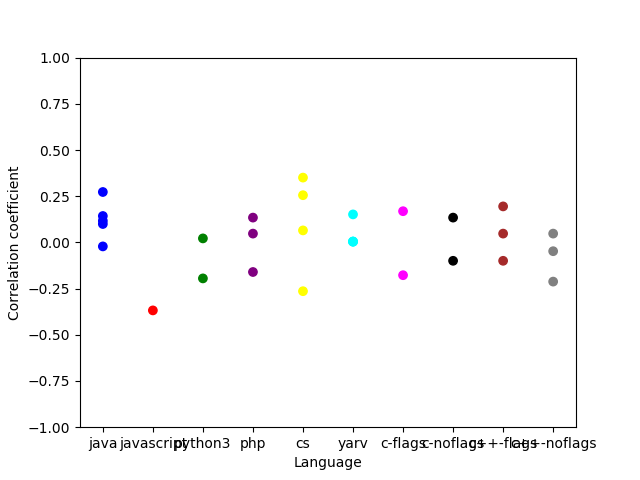
\includegraphics[width=.6\textwidth]{graphs/kendall_Binarytrees.png}
    \caption{The Kendall correlation score for every single program that solves the Binarytrees problem.}
    \label{fig:corr-binarytrees}
\end{figure}

\begin{figure}[h]
    \centering
    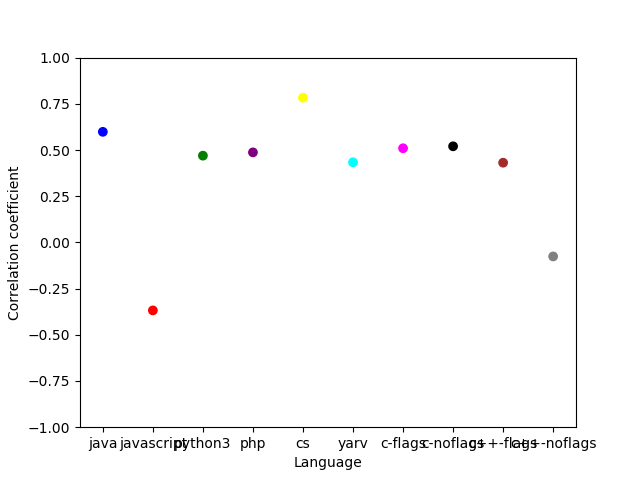
\includegraphics[width=.6\textwidth]{graphs/kendall-lang_Binarytrees.png}
    \caption{The Kendall correlation score for every programming language that solves the Binarytrees problem.}
    \label{fig:corr-lang-binarytrees}
\end{figure}

\begin{figure}[h]
    \centering
    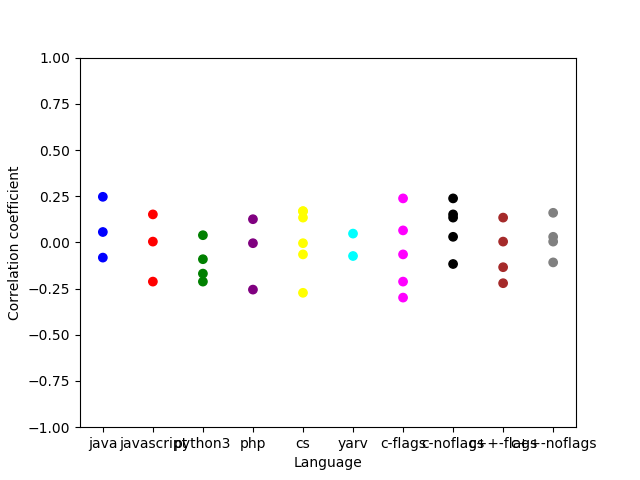
\includegraphics[width=.6\textwidth]{graphs/kendall_Fannkuchredux.png}
    \caption{The Kendall correlation score for every single program that solves the Fannkuchredux problem.}
    \label{fig:corr-fannkuchredux}
\end{figure}

\begin{figure}[h]
    \centering
    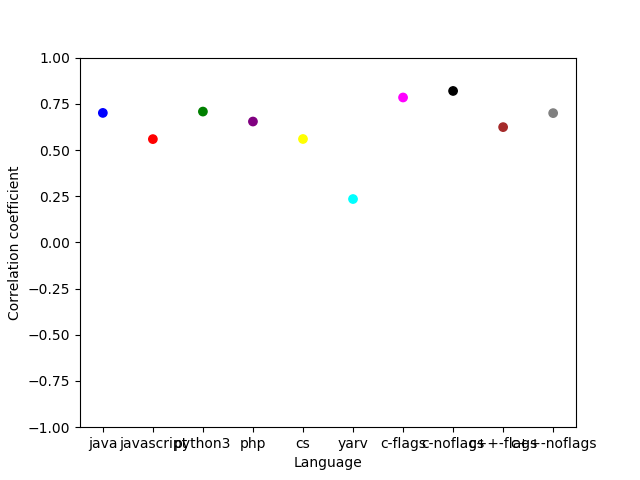
\includegraphics[width=.6\textwidth]{graphs/kendall-lang_Fannkuchredux.png}
    \caption{The Kendall correlation score for every programming language that solves the Fannkuchredux problem.}
    \label{fig:corr-lang-fannkuchredux}
\end{figure}

\begin{figure}[h]
    \centering
    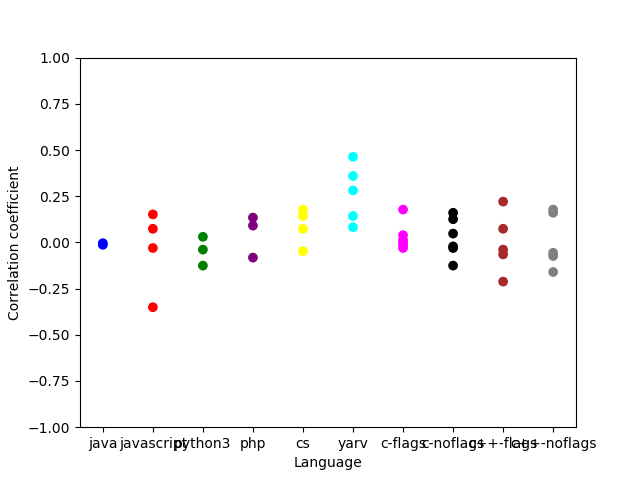
\includegraphics[width=.6\textwidth]{graphs/kendall_Fasta.png}
    \caption{The Kendall correlation score for every single program that solves the Fasta problem.}
    \label{fig:corr-fasta}
\end{figure}

\begin{figure}[h]
    \centering
    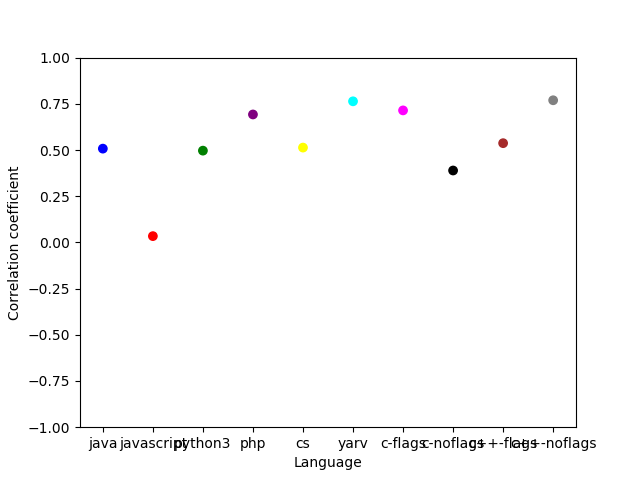
\includegraphics[width=.6\textwidth]{graphs/kendall-lang_Fasta.png}
    \caption{The Kendall correlation score for every programming language that solves the Fasta problem.}
    \label{fig:corr-lang-fasta}
\end{figure}

\begin{figure}[h]
    \centering
    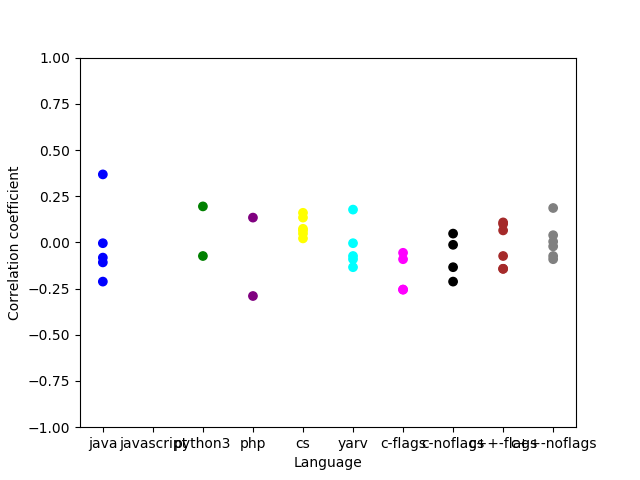
\includegraphics[width=.6\textwidth]{graphs/kendall_Mandelbrot.png}
    \caption{The Kendall correlation score for every single program that solves the Mandelbrot problem.}
    \label{fig:corr-mandelbrot}
\end{figure}

\begin{figure}[h]
    \centering
    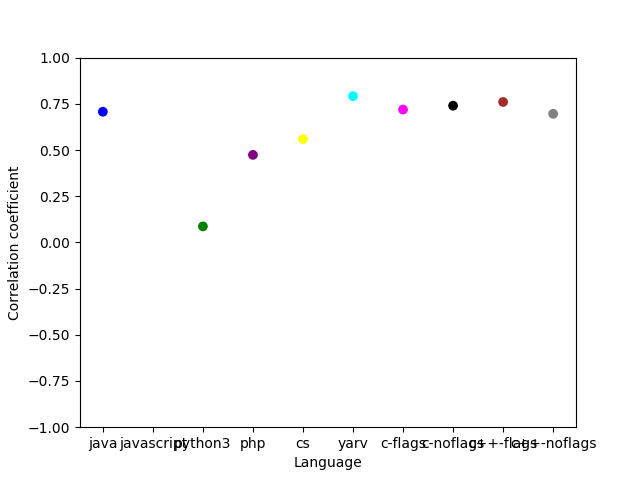
\includegraphics[width=.6\textwidth]{graphs/kendall-lang_Mandelbrot.png}
    \caption{The Kendall correlation score for every programming language that solves the Mandelbrot problem.}
    \label{fig:corr-lang-mandelbrot}
\end{figure}

\begin{figure}[h]
    \centering
    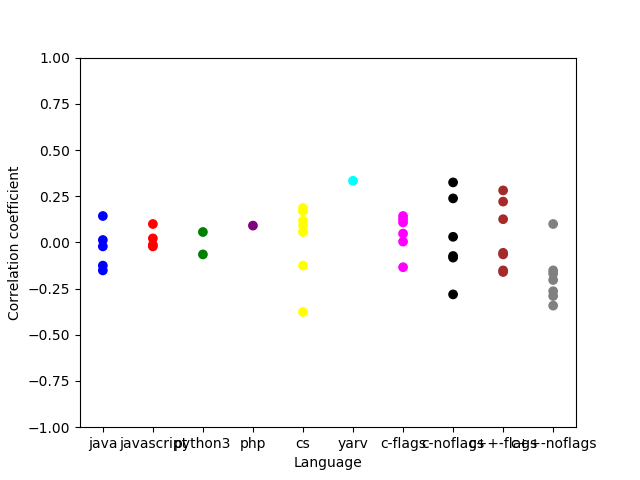
\includegraphics[width=.6\textwidth]{graphs/kendall_Nbody.png}
    \caption{The Kendall correlation score for every single program that solves the Nbody problem.}
    \label{fig:corr-nbody}
\end{figure}

\begin{figure}[h]
    \centering
    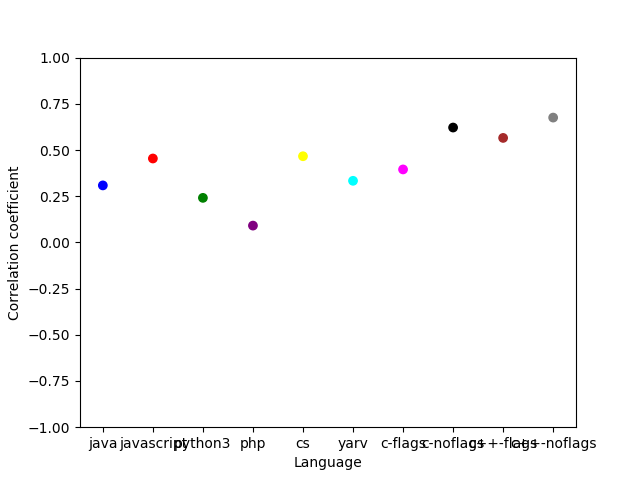
\includegraphics[width=.6\textwidth]{graphs/kendall-lang_Nbody.png}
    \caption{The Kendall correlation score for every programming language that solves the Nbody problem.}
    \label{fig:corr-lang-nbody}
\end{figure}

\begin{figure}[h]
    \centering
    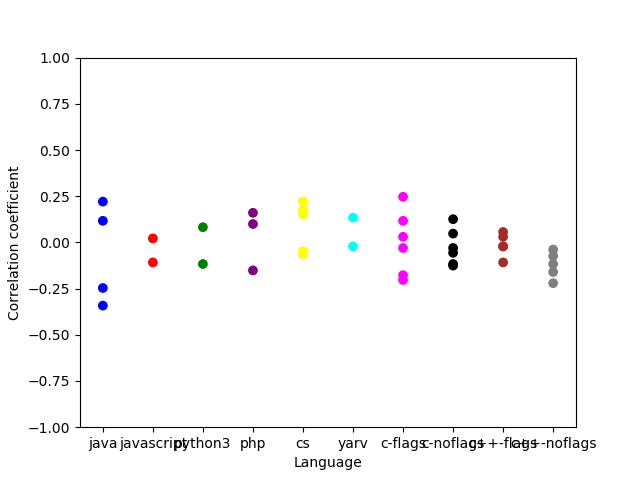
\includegraphics[width=.6\textwidth]{graphs/kendall_Revcomp.png}
    \caption{The Kendall correlation score for every single program that solves the Revcomp problem.}
    \label{fig:corr-revcomp}
\end{figure}

\begin{figure}[h]
    \centering
    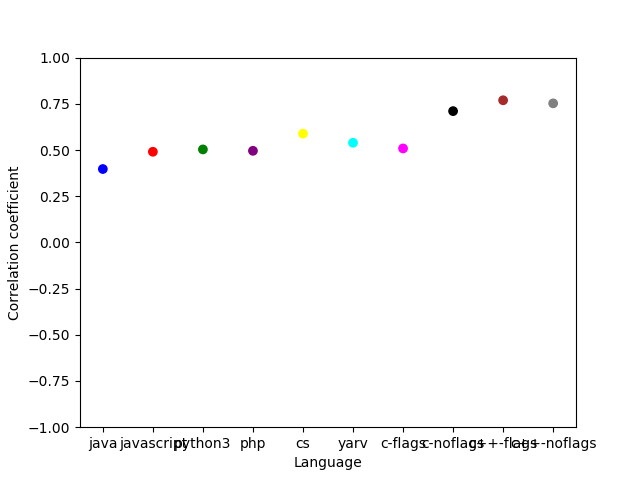
\includegraphics[width=.6\textwidth]{graphs/kendall-lang_Revcomp.png}
    \caption{The Kendall correlation score for every programming language that solves the Revcomp problem.}
    \label{fig:corr-lang-revcomp}
\end{figure}

\begin{figure}[h]
    \centering
    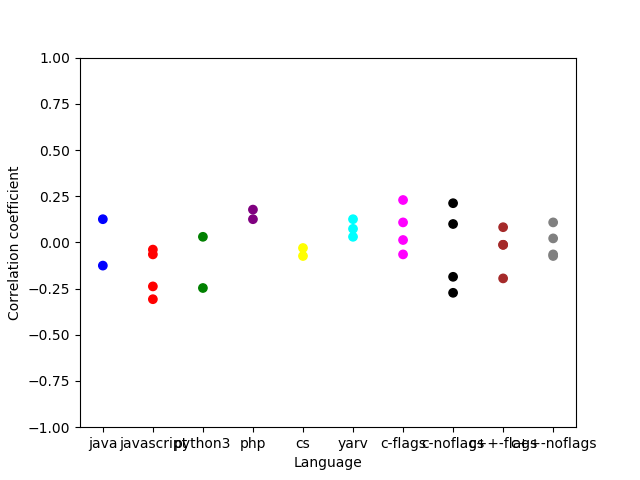
\includegraphics[width=.6\textwidth]{graphs/kendall_Spectralnorm.png}
    \caption{The Kendall correlation score for every single program that solves the Spectralnorm problem.}
    \label{fig:corr-spectralnorm}
\end{figure}

\begin{figure}[h]
    \centering
    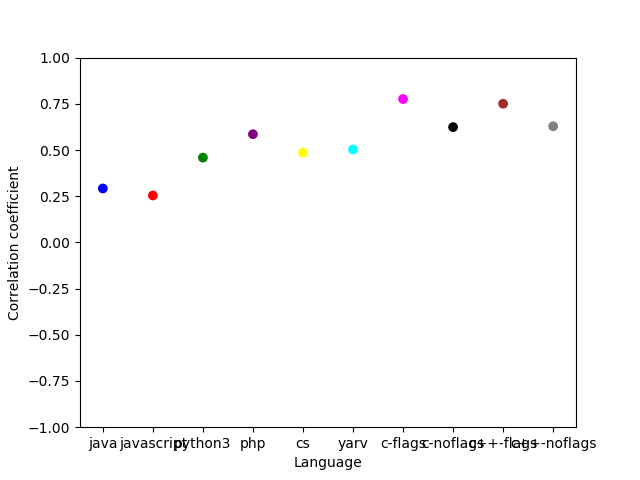
\includegraphics[width=.6\textwidth]{graphs/kendall-lang_Spectralnorm.png}
    \caption{The Kendall correlation score for every programming language that solves the Spectralnorm problem.}
    \label{fig:corr-lang-spectralnorm}
\end{figure}

\end{appendices}